
\section{Introduction}

The Semantic Web is a big container, a universal medium for data, information
and knowledge exchange. But the Semantic Web is not only about putting data on
the Web, it is something more. There are necessary some basic rules to follow
in order to get a useful knowledge from all this linked data. Tim Berners-Lee 
outlined four principles~\cite{TimBL2006} that could be summarized as that you 
must use \texttt{URIs}~\cite{RFC3986} as names and provide useful information 
where you could be discovered more information. But cool URIs~\cite{Sauermann2007} 
are not enough, you also need to provide the best representation expected for 
each agent, human or software, request.

The HTTP Protocol~\cite{HTTP} is used to request representations of Web documents
and send back the responses. It provides a mechanism known as \textit{content negotiation}.
Using this mechanism it is possible to offer Web content in different formats and
languages. Use transparent content negotiation in HTTP~\cite{Holtman1998} has many 
benefits~\cite{Seshan1998}, but must be implemented carefully if you do not want 
to make some mistakes, as we could see with more detail in next sections of this
paper.

\section{Content negotiation with Apache: Recipes}

Apache HTTP Server, probably the most used Web server now, mainly provides three ways 
to implement content negotiation\footnote{\url{http://httpd.apache.org/docs/2.0/content-negotiation.html}}, 
each one with a different approach:

\begin{itemize}

  \item \textbf{Type Map:} explicit handlers described in a file (.var) for each 
        resource. The necessary configuration is quite complicated and tedious, 
        so probably that is the reason because it is hardly used.

  \item \textbf{MultiViews:} based in the MIME-type of the files, MultiViews 
        delegates in Apache the task of choosing the best file in the current 
        directory to serve when the resource requested does not exist. It adds 
        an additional header (\texttt{Content-Location}) indicating the direct 
        location of the file served. Could also be extended using 
        \texttt{mod\_mime}\footnote{\url{http://httpd.apache.org/docs/2.0/mod/mod_mime.html}}
        to associate concrete handlers to other file extensions.

  \item \textbf{Rewrite request:} probably because the both methods previously 
        presented do not work as expected, the most currently used is another 
        that is not designed specifically for content negotiation tasks. This
        mechanism uses the module 
        \texttt{mod\_rewrite}\footnote{\url{http://httpd.apache.org/docs/2.0/mod/mod_rewrite.html}}
        to rewrite the request according some mandatory ad-hoc rules and redirect,
        using HTTP \texttt{30X} status codes, to the appropriate URI. Obviously it loses 
        some time with the extra HTTP round-trip, but it is negligible.

\end{itemize}

The W3C has published \textit{Best Practice Recipes for Publishing RDF Vocabularies}~\cite{Recipes},
a document with several recipes that show how to publish RDF/OWL Vocabularies using
the last mechanism described. It provides step-by-step instructions for publishing 
vocabularies on the Web, giving example configurations designed to cover the most 
common cases. It's a document really useful to help to publish the vocabularies.

But it is not perfect, ant still there is an important issue to 
solve\footnote{\url{http://www.w3.org/2006/07/SWD/track/issues/58}}: 
``the recipe for responding to an accept header only responds to a header which
EXACTLY matches''. Consider cases like \texttt{application/rdf+xml;q=0.1} or 
\texttt{text/*} or combinations of such patterns. This is a very serius problem
with not an easy solution. Probably might be solved by moving from \texttt{mod\_rewrite}
to \texttt{mod\_negotiation}, or with a combination of both techniques.

\textbf{FIXME: solution ISSUE 58???}
%http://lists.w3.org/Archives/Public/public-swd-wg/2007Jul/0177.html

\section{Vapour, a scripting approach to debug content negotiation} %find a better title for this section

As we can see, the Recipes are not perfect. And testing the results of content 
negotiation can become fairly complex for some of their. Obviously you could do 
it manually or using some tools, such as 
cURL\footnote{Richard Cyganiak's explanation of how to use cURL to debug content negotiation, 
blog post available at: \url{http://dowhatimean.net/2007/02/debugging-semantic-web-sites-with-curl}}.
But it is not a very handy way, specially when you need to do intensive tests over your 
configuration.

In order to facilitate the testing of the results of content negotiation on a single 
URI, we developed a web-based application called Vapour\footnote{\url{http://vapour.sourceforge.net/}} 
that facilitates the task. This service will request a provided URI from a server, 
run a test suite specifically designed to test the response of the server against 
the Recipe specifications. According with these tests, the system suggest you the 
best recipe for your server configuration. It is build upon a RDF Store (in memory) 
where all asserts are stored. It uses a combination of EARL~\cite{EARL}, HTTP
Vocabulary~\cite{Koch2007}, a RDF representation of the Recipes and three small 
properties created specifically for this purpose. So Vapour could provide 
reports both in HTML and in RDF. For (X)HTML view the service displays a 
pretty and intuitive pass/fail report on each set of tests as  well as a detailed 
explanation of its  findings (Figure~\ref{fig:report-summary}).
For RDF view %,obviously using content negotiation (FIXMEEEEEEEEEEEEEEEEEE)
the system provide a RDF/XML serialization of the report. So it could be easy 
to deploy another service that check the compliance of a specific collection 
of vocabularies published on the Web.

\begin{figure}
 \centering
 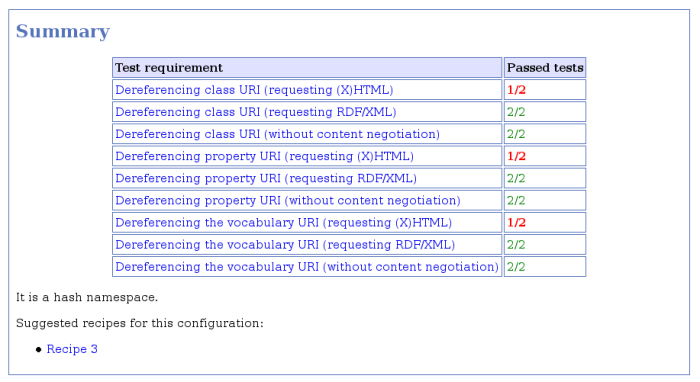
\includegraphics[width=12cm]{images/report-summary.png}
 \caption{\label{fig:report-summary}Vapour report summary.}
\end{figure}

The application has been developed in the Python scripting language, using common
python libraries such as urllib, httplib, web.py and RDFLib, Its source code is 
also available in the project web page as opensource under the terms of W3C Software 
License.

FIXME: more about python and scripting

\begin{figure}
 \centering
 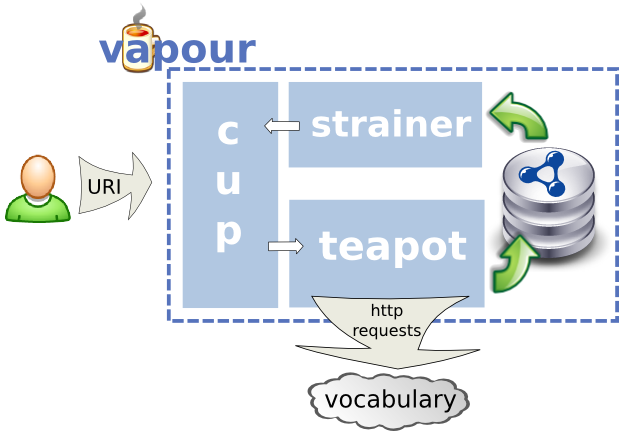
\includegraphics[width=12cm]{images/arch.png}
 \caption{\label{fig:arch}Hight level architecture of Vapour.}
\end{figure}

As it can be viewed in the Figure~\ref{fig:arch}, Vapour is composed for three 
components: FIXME

\begin{itemize}

  \item \textbf{cup:} implements the web interface FIXME

  \item \textbf{teapot:} implementes the Recipes and all the HTTP dialogs FIXME

  \item \textbf{strainer:} implements the reports FIXME

\end{itemize}

FIXME: arch diagram

FIXME

FIXME: something about security?

An online demo of the project it available at: 
\begin{center}\url{http://idi.fundacionctic.org/vapour}\end{center}

\section{Conclusions}

Content negotiation is difficult, scripting languages are useful to solve these kind on tasks, etc...

FIXME

